% This file is for chapter 3

\chapter{Revisiting Parallel Portfolio Selection with KL Divergence}


\section{Introduction}

Algorithms designed to solve combinatorial problems often exhibit complementary performance across different problem instances. Therefore, using a portfolio of algorithms frequently demonstrates superior performance compared to selecting the single best solver (SBS) averaged across all instances \cite{Huberman1997,GOMES200143}. Portfolios can either be run in parallel, or a single algorithm can be selected on an instance-by-instance basis by training performance models using machine learning algorithms. However, both methods have drawbacks. 

Algorithm selection has proven to be effective in solving different problems such as SAT, constraint programming, and mixed integer programming, as demonstrated by systems such as SATzilla, Hydra, and AutoFolio \cite{satzilla,lindauer2015autofolio,cphydra,XuEtAl11}. In single algorithm selection, if machine learning models are not well generalized, they might not select the correct best algorithm for a given instance. Although executing the whole portfolio of algorithms seems to avoid this issue, the more solvers that perform computations in parallel, the more time-out computations we will encounter \cite{pmlr-v140-kashgarani21a,LINDAUER2017272}. However, the proposed parallel portfolio approaches often simulate parallel execution based on sequential data, which conceals the significant overhead and performance drop that occurs when many algorithms run parallel. 

Based on the results presented in the third chapter, even with a small number of solvers, selecting a single algorithm using the imperfect regression random forest ML model can outperform parallel portfolios \cite{pmlr-v140-kashgarani21a}. In Chapter 4, we proposed a hybrid approach that leverages both algorithm selection and parallel execution. We introduced a middle-path strategy that identifies the most promising subset of algorithms to run simultaneously on a single non-distributed computer \cite{kashgarani2023automatic}. This innovative method demonstrated improved performance by utilizing three regression random forest algorithm selectors with different implementations and uncertainty estimation methods.

Using the method proposed in the previous chapter, it is possible to select an instance-based subportfolio of solvers to run in parallel, avoiding the drawbacks of algorithm selection and reducing the overhead associated with running too many solvers simultaneously. This method can achieve optimal or near-optimal performance, provided the virtual best solver is included in the selected subset of algorithms. We used the estimated uncertainty of the predictions while considering the impact of overhead from running the portfolio in parallel. 

However, this strategy still has some limitations. Specifically, the threshold value $p_{\cap}$--which is defined as the threshold for the joint probability between the prediction distributions of the minimum predicted algorithm and other algorithms, and serving as a measure of the likelihood that an algorithm is predicted to perform very closely to the minimum predicted algorithm—could not be generalized across all scenarios and algorithm performance models, as the tuned values varied significantly. Here, we aim to provide an alternative formulation for subportfolio selection that overcomes this limitation.

In this chapter, we revisit the method of selecting the optimal parallel subportfolio of algorithms to run on a single computing machine. Similar to the main proposed method, we incorporate the uncertainty of the performance predictions. Here, rather than using the threshold $p_\cap$ in Equation~\ref{eq:7} as an estimate of the probability that the algorithm is as good as the best predicted algorithm, we investigated the use of the Kullback–Leibler (KL) divergence method, which measures the difference between the probability distributions of the predicted algorithms. This method provides an understanding of the differences between algorithm predictions, in contrast to the joint probability approach, which focused on the similarity of predictions. This enables a redefined selection criterion based on the divergence from the best-predicted performance distribution.



\section{Revisit Parallel Portfolio Selection}

We aim to select a subset of solvers \begin{math} P_i \subseteq S \end{math} for a given instance \(i \in I\), prioritizing algorithms predicted to perform best (\( A \in S \) and \( A \in P_i \)) based on their predicted performance \(\hat{m}\). For each instance, a total ranking of algorithms in the portfolio \(S\) is established using their predicted performance:

\[
A < B \quad \text{if} \quad \hat{m}(A, i) < \hat{m}(B, i); A, B \in S
\]

From this ranking, the rank \(r_{A, i}\) is assigned to each algorithm \(A\), representing the number of algorithms predicted to outperform \(A\) on instance \(i\). A portfolio of size \(n\) is then defined by the top \(n\) ranked algorithms:

\[
P_i = \{A \in S \: | \: r_{A,i} \leq n\}
\]

This method allows the selection of a subset of solvers for parallel execution, balancing the likelihood of including the best-performing solver with the overhead of running multiple solvers. However, the critical challenge in parallel portfolios is determining the appropriate portfolio size $n$ for each problem instance. To address this balance, we incorporate the predicted performance distribution of algorithms and their associated uncertainty. 

Similar to the proposed method in Chapter 4, instead of considering only a point prediction, we consider the predicted distribution of performance metric values, characterized by its mean and standard deviation. Formally, we denote the standard deviation of the prediction \begin{math}\hat{m}(A, i)\end{math} as \begin{math}\sigma_{A, i}\end{math} for each solver $A$ and instance $i$. We assume that the predictions of our performance models follow a normal distribution, i.e. the predicted value is the mean of that distribution, and allow us to characterize it completely together with the standard deviation. In the previous approach, we assess the likelihood that two algorithms perform equally well by calculating the overlap area between their prediction distributions. If two algorithms are predicted to perform very similarly, then the overlap area between the distributions will be very large. Here, we replace this method by considering the Kullback–Leibler (KL) divergence between the two univariate Gaussian distributions. KL divergence captures the divergence in shape and spread between the distributions.

We are in particular interested in the predicted performance distribution of the best-predicted algorithm $A_{1,i}$ (no algorithms are predicted to perform better than it), and how the predictions for the other algorithms compare to it. Formally, for the best predicted solver $A_{1,i}$ on instance $i$ the distribution of predictions is \begin{math} \hat{m}(A_{1,i}, i) \sim \hat{M}(\mu_{A_{1,i},i}, \sigma^2_{A_{1,i},i}) \end{math} with probability density function \begin{math} f_{A_{1,i},i}\end{math} and cumulative distribution function \begin{math} F_{A_{1,i},i}\end{math}. The performance distributions for other algorithms are defined similarly.

The Kullback–Leibler (KL) divergence is a statistical metric used to quantify the difference between two probability distributions \cite{KL}. According to the formulation in \cite{bishop2006pattern}, given two distributions $p$ and $q$ with probability density functions $p(x)$ and $q(x)$, the KL divergence is calculated as:

\begin{equation}\label{eq:5.4}
    KL(p \| q) = - \int p(x) \log q(x) \, dx + \int p(x) \log p(x) \, dx
\end{equation}

In our context, we are interested in comparing the predicted performance distributions of two algorithms, $A_{x}$ and $A_{y}$, on a specific instance $i$. Let $f_{A_{x},i}$ and $f_{A_{y},i}$ denote the probability density functions of the predicted performance of algorithms $A_{x}$ and $A_{y}$ on instance $i$, respectively. By substituting $p(x)$ with $f_{A_{x},i}$ and $q(x)$ with $f_{A_{y},i}$, we adapt the KL divergence to quantify the difference in predicted performance between the two algorithms. Thus, the KL divergence between the performance distributions of $A_{x}$ and $A_{y}$ in instance $i$ is computed as follows:

\begin{equation}\label{eq:5.5} KL(f_{A_{x},i} \| f_{A_{y},i}) = - \int f_{A_{x},i}(x) \log f_{A_{y},i}(x) dx + \int f_{A_{x},i}(x) \log f_{A_{x},i}(x) dx \end{equation}

This formulation indicates to what extent the probability distributions differ. Since the two distributions are univariate Gaussians, the exact formula for KL divergence is as follows (we omit the index $i$ for the sake of brevity here):

\begin{equation}\label{eq:5.6}
    KL(f_{A_x} \| f_{A_y}) = \log \frac{\sigma_{A_y}}{\sigma_{A_x}} + \frac{\sigma_{A_x}^2 + (\mu_{A_x} - \mu_{A_y})^2}{2 \sigma_{A_y}^2} - \frac{1}{2}
\end{equation}

We define $kl \in [0, \infty)$ as a threshold for the computed KL divergence to include a given algorithm:

\begin{equation}\label{eq:5.7}
 P_i = \{A \:| \:  KL(f_{A_{1,i},i} \| f_{A_{x,i},i}) \leq \\kl\:\}
\end{equation}

$kl$ is 0 for the best predicted algorithm. In contrast to $p_{\cap}$, which could only be in the range of [0,1], the value of $kl$ can be greater than 1. A very large value of $kl$ corresponds to algorithms whose distributions diverge the most from that of the best predicted algorithm, that is, algorithms with performance predictions that are markedly different from those of the best predicted algorithm.

We can adjust the size of the parallel portfolio by modifying the $kl$ threshold. When $kl$ is set to 0, only the best predicted algorithm and those expected to perform identically are included. Setting $kl$ to a very large positive value allows all algorithms to be included. Finding the optimal $kl$ is necessary to determine how many solvers to include in the portfolio. This flexibility enables us to tailor the approach to specific algorithm selection scenarios, allowing the selection of algorithms to run in parallel and accommodating any potential inaccuracies in performance predictions.

\section{Experimental Setup}
\subsection{Data Collection}

We used the same five scenarios as in the previous chapter \cite{kashgarani2023automatic}, now included in the ASlib benchmark repository \cite{BISCHL201641}: MAXSAT19-UCMS, SAT11-INDU, SAT18-EXP, SAT16-MAIN, and IPC2018. These datasets include algorithm performance data from single and parallel runs, with parallel run measurements conducted on individual machines as described in \cite{kashgarani2023automatic}. Feature extraction was performed using the SATZilla feature extraction code for MAXSAT19-UCMS, SAT11-INDU, SAT16-MAIN, and SAT18-EXP, producing 54 features, while IPC2018 features were extracted using the code from \cite{Fawcett_Vallati_Hutter_Hoffmann_Hoos_Leyton-Brown_2014}, resulting in 305 features.

\subsection{Training}
We used the same random forest regression models from Chapter 4. The random forest regression models are trained in three ways: one using the randomForest package in R and two using the Ranger package, to predict algorithm performance on specific instances. Random forests are generally recognized for their strong performance in algorithm selection and performance prediction \cite{BISCHL201641,HUTTER201479}. Given the existence of two distinct implementations, we trained the models using both \textit{randomForest} and \textit{Ranger} implementations.

Our regression random forest models are built using the MLR package with the randomForest package as dependency, and the Ranger models are trained using the MLR3 and Ranger implementations. These models predict the runtime for each solver as the mean of the underlying distribution and estimate the standard deviation. The initial random forest model and one of the Ranger models use the Jackknife method \cite{wager2014confidence, mlr}. 
The Jackknife method estimates the standard deviation of the mean predictions in all observations used to train the random forest. This technique involves training the random forest model on $n-1$ observations, leaving one out each time to make a prediction, and repeating this for each observation. The mean prediction for each tree is calculated by averaging its predictions on the left-out data points. The Jackknife method assumes that predictions follow a normal distribution, with the standard deviation indicating the uncertainty of the overall prediction. The infinitesimal jackknife method assesses the impact of each observation by slightly down-weighting it, unlike the traditional jackknife, which removes one observation at a time.

Our setup closely follows the approach in \cite{BISCHL201641} for all three models: we excluded instance features with constant values and imputed missing feature values by using the mean of all nonmissing values for each feature. The random forest hyperparameters were tuned through random search with 250 iterations, where $ntree$ was varied from 10 to 200 and
$mtry$ from 1 to 30, using nested cross-validation with three inner folds and 10 outer folds \cite{BISCHL201641}.

\subsection{Tuning $kl$ and $p_{\cap}$}

\begin{table}
\centering
\caption{Optimum value of $kl$ for each benchmark and model.}
\label{tab:kl}
\begin{tabular}{p{3.6cm} cccc}
\toprule
Scenario & RandomForest\_Jackknife & Ranger\_Jackknife & Ranger\_Inifinitesimal\\
\midrule
IPC2018 & 0.71 & 2.35 & 2.39 \\
MAXSAT19-UCMS & 0.63 & 2.7 & 2.7\\
SAT11-INDU & 0.55 & 1.62 & 1.94\\
SAT16-MAIN & 2.66 & 2.06 & 2.96\\
SAT18-EXP & 0.12 & 1.81 & 1.35\\
\midrule
Generic best & 0.41 & 2.65 & 2.82\\
\bottomrule
\end{tabular}
\end{table}

The tuned $p_{\cap}$ value for each benchmark and each random forest model is listed in Table \ref{tab:pcap} and we are using the same values in this chapter. These values were individually optimized for each scenario to ensure that the selected portfolio provided the best balance between performance and computational efficiency. For tuning $kl$, we perform a grid search to determine the optimal value in Equation~\ref{eq:5.7} for each scenario. The search is carried out over the interval $[0, 3)$ with a resolution $0.01$, resulting in 300 possible values. 

The tuned $p_{\cap}$ value for each benchmark and each random forest model is listed in Table \ref{tab:pcap}, and we use the same values in this chapter. These values were individually optimized for each scenario to ensure that the selected portfolio provided the best balance between performance and computational efficiency. For tuning $kl$, we perform a grid search to determine the optimal value in Equation~\ref{eq:5.7} for each scenario. The search is carried out over the interval $[0, 3)$ with a resolution of 0.01, resulting in 300 possible values.

\subsection{Baselines}

For all the comparisons mentioned, we evaluate the performance of our approaches against several baseline methods. Specifically, we compare to the sequential virtual best solver (VBS), which picks the best solver for each problem instance with a cumulative misclassification penalty of zero, and to the sequential single best solver (SBS), which is the solver with the best average performance across all instances and a cumulative misclassification penalty of one. For parallel runs, the VBS is the best solver for each instance but includes the overhead for $n$ parallel runs. The parallel SBS is determined similarly, using the solvers with the best average performance instead of the best for each instance. We executed multiple solvers in parallel to capture the real run-time of the best solver in this setup, instead of assuming that it would run sequentially.

We have three algorithm selectors: RFJ (random forest with Jackknife), RJ (Ranger with Jackknife), and RI (Ranger with infinitesimal Jackknife). Each algorithm selector has five approaches for comparison. The first involves selecting algorithms on a per-instance basis, running the top $n$ predicted algorithms in parallel without accounting for any uncertainty the subportfolio selection approaches. Using the notation introduced in the previous chapter, we assign $p_{\cap}=0$ and limit the number of runs to match the available processors. Also, when we assign $kl = \infty$, we are doing the same thing and limiting the number of runs to match the available processors. The second approach uses the associated tuned $p_{\cap}$ values mentioned in Table~\ref{tab:pcap}. The third approach uses the average $p_{\cap}$ value, which was the best generic value across all scenarios. Other approach uses the associated tuned $kl$ values mentioned in Table~\ref{tab:kl} for each scenario and performance model. The last approach uses the generic best $kl$ value across all scenarios for each performance model.

We evaluate the proposed method by measuring the penalized average runtime with a factor of 10 (PAR10), the misclassification penalty (MCP), and the runtime. The PAR10 metric equals the actual runtime if the algorithm successfully solves the instance within the timeout; otherwise, it is calculated as the timeout multiplied by 10. The MCP represents the difference between the performance of the selected algorithm and that of the optimal algorithm. The mean and standard deviation of these values are presented in Tables~\ref{tab:summary5-ipc-max},\ref{tab:summary5-sat11-sat16}, and\ref{tab:summary5-sat18}. We normalize PAR10 values across scenarios using the performances of the VBS and SBS, reporting the proportion of the performance gap each approach bridges. On this normalized scale, 0 denotes the performance of the SBS, while 1 denotes the performance of the VBS. 

In the tables, we report the mean and standard deviation of the normalized gap closed across the 10 folds of data used to train the performance models. In contrast to the reported runtime, MCP, and PAR10 scores, where we present the mean and standard deviation across the distribution of all instances. We use folds here to avoid zero denominators in cases where the single best solver is the actual best solver for an instance, based on the normalized gap closed formula $\frac{\text{sbs} - \text{approach}}{\text{sbs} - \text{vbs}}$. The plots~\ref{fig:all_results}, show the PAR10 score normalized gap closed over the entire distribution of instances.

\section{Results}
\subsection{Tuning of $kl$ and $p_{\cap}$}

Tuning $p_{\cap}$ and $kl$ reveals that the optimal values vary by scenario. Tables~\ref{tab:pcap} and~\ref{tab:kl} present the optimal values for each scenario and algorithm selector. We presented Figure~\ref{fig:kl_sensitivity}, which shows the normalized gap closed for the mean, 25th percentile, 50th percentile, and 75th percentile across each scenario based on $kl$ value. Although optimal values vary significantly between scenarios and performance models, normalized gaps closed remain relatively small as long as $kl$ is not too low. For the most optimal performance, we recommend tuning $kl$ for each specific scenario.

The optimal value of $kl$, similar to $p_{\cap}$, provides insight into the predictive accuracy of the performance models. A large $kl$ value suggests that the models' predictions may lack accuracy, as it requires including solvers whose predicted runtime distributions differ significantly from that of the best predicted solver in order to capture solvers that perform well. If the optimal value of $kl$ were 0, we would include only solvers that are exactly similar to the best-predicted solver. A very large optimal $kl$ requires us to include all solvers, even those whose predicted distributions differ entirely from the best predicted solver. 

Here, the optimal values for $kl$ are relatively small, typically up to 2.5 in most cases. The further the $kl$ value deviates from 0, the lower the accuracy. Table~\ref{tab:kl} also shows that the RFJ model, which uses randomForest with a Jackknife uncertainty estimate, has a significantly lower optimal $kl$ in most scenarios, suggesting that this model should outperform the other two when selecting single solver in 4 out of 5 scenarios in terms of prediction accuracy. This is confirmed by Tables~\ref{tab:summary5-ipc-max}, \ref{tab:summary5-sat11-sat16} and~\ref{tab:summary5-sat18} which is denoted as $AS (RFJ)$. The optimal $kl$ values are closer for all scenarios when we have a single model. This seems to contrast with $p_{\cap}$, where different scenarios had significantly varying values per model. Here, the values are more consistent, suggesting that tuning this parameter per model should yield good performance.

\subsection{$AS_{p_{\cap}}$ vs. $AS_{kl}$ Comparison}

To evaluate the effectiveness of any of the approaches, we carried out a series of experiments using the optimum best value for $p_{\cap}$ and $kl$ and $p_{\cap} = 0$ for each scenario, where we varied the number of processors used for parallel execution from one to ten for the scenarios SAT18-EXP, SAT16-MAIN, SAT11-INDU and IPC2018. For the MAXSAT19-UCMS scenario, we used a maximum of seven processors, as there are only seven algorithms. Figure~\ref{fig:klvspcap} shows the PAR10 score results in terms of the normalized performance gap closed between the sequential single best solver and the sequential virtual best solver for all scenarios and number of processors. In addition, Tables~\ref{tab:summary5-ipc-max},~\ref{tab:summary5-sat11-sat16} and~\ref{tab:summary5-sat18} show the mean and standard deviation values for runtime, MCP and PAR10 when limiting the maximum number of parallel runs to 10 or SAT18-EXP, SAT16-MAIN, SAT11-INDU and IPC2018, and to 7 for MAXSAT19-UCMS. In addition, we reported the mean and standard deviation of the normalized gap closed across folds in these tables. This differs from the plots, as the plots report values in terms of the mean of the problem distribution rather than across folds.

Here, we discuss the results of the comparison of $AS_{p_{\cap}}$ with the $AS_{kl}$ methods. For this comparison, we excluded the results of the RJ model in Figure~\ref{fig:klvspcap} because, as mentioned in the previous section comparing ranger and randomForest, the RJ model did not outperform the other two models in subportfolio selection, while RI and RFJ were competitive in portfolio selection. This is also evident in Tables~\ref{tab:summary5-ipc-max}, \ref{tab:summary5-sat11-sat16}, and~\ref{tab:summary5-sat18} that the RJ model did not surpass the other two when using $AS_{p_{\cap}}$ and $AS_{kl}$. Therefore, we discuss the results for the RI and RFJ models when selecting subportfolios using Equation~\ref{eq:7}, denoted as $AS_{p_{\cap}}$, and Equation~\ref{eq:5.7}, denoted as $AS_{kl}$.

When comparing $AS_{p_{\cap}}$ and $AS_{kl}$ with optimal threshold values, based on Tables~\ref{tab:summary5-ipc-max}, \ref{tab:summary5-sat11-sat16}, and~\ref{tab:summary5-sat18}, $AS_{kl}$ outperforms $AS_{p_{\cap}}$ in three of four performance metrics for IPC2018 and the RFJ model. For the RI model, $AS_{p_{\cap}}$ is superior in three of the four metrics, while for the RJ model, $AS_{kl}$ performs worse in all performance metrics. Figure~\ref{fig:klvspcap} further illustrates that $AS_{p_{\cap}}$ consistently outperforms $AS_{kl}$ for both the RFJ and RI models when the cores are limited to different values. For the MAXSAT19-UCMS and SAT11-INDU scenarios, $AS_{p_{\cap}}$ performs better than $AS_{kl}$ in all performance metrics for the RJ, RFJ, and RI models, which is also reflected in the closed mean normalized gap in Figure~\ref{fig:klvspcap}. In the SAT16-MAIN scenario, $AS_{p_{\cap}}$ is overall superior, except for the RFJ model, where both methods perform equally, and the RJ model where the normalized gap closed for folds is slightly worse for $AS_{p_{\cap}}$. In the SAT18-EXP scenario, $AS_{p_{\cap}}$ generally outperforms $AS_{kl}$, except for the RFJ model where the two are highly competitive. In three of four performance metrics, $AS_{kl}$ is better, while $AS_{p_{\cap}}$ excels in the remaining metric.

When comparing the RFJ and RI models for portfolio selection using the $AS_{kl}$ method, the RFJ model performed consistently best in all scenarios. This contrasts with the $AS_{p_{\cap}}$ approach, where the RI model outperformed the RFJ model in two out of five scenarios. When comparing $AS_{p_{\cap}}$ and $AS_{kl}$ using the generic best values across the tuned scenarios for each model, $AS_{p_{\cap}}$ outperforms $AS_{kl}$ in two of the three models for IPC2018, MAXSAT19-UCMS and SAT16-MAIN. However, for the RFJ model in these scenarios, the trend is reversed, with $AS_{kl}$ performing slightly worse. For SAT11-INDU and SAT18-EXP, $AS_{p_{\cap}}$ is the consistently better approach across all models.

When comparing all the experimented methods in all scenarios with the number of parallel runs limited to 10, the $AS_{p_{\cap}}$ of the RI model delivered the best performance for IPC2018 and SAT11-INDU in terms of runtime, MCP, normalized gap, and PAR10. For these scenarios, $AS_{kl}$ of the RI model was the second-best method. For MAXSAT19-UCMS, the $AS_{p_{\cap}}$ of the RFJ model achieved the best performance, followed by the $AS_{kl}$ of the RFJ model as the second-best method. In SAT16-MAIN, $AS_{p_{\cap}}$ of the RI model, with $p_{\cap}$ set to zero and selecting the top 10 predicted algorithms, emerged as the best method. The second-best method in this scenario was the $AS_{p_{\cap}}$ of the RI model, using the generic best value for $p_{\cap}$. Finally, for SAT18-EXP, the $AS_{p_{\cap}}$ and $AS_{kl}$ methods of the RFJ model performed very competitively, both achieving the best performance. 

Although the $AS_{p_\cap}$ method appears to be in general superior to $AS_{kl}$, its performance is very close, making $AS_{kl}$ the best alternative in the absence of $AS_{p_\cap}$. One significant advantage of $AS_{kl}$ is that the tuned values of $kl$ for different scenarios are highly consistent, and this suggests that tuning of $kl$ globally across all scenarios can still produce good performance. This consistency reduces the cost of scenario-specific tuning. In contrast, the $p_{\cap}$ values vary significantly between different models, and it makes tuning more challenging and model-dependent. On the other hand, $kl$ demonstrates greater consistency, with its best generic values for the RI and RJ models being close, which further highlights its practicality for streamlined optimization.

\begin{figure}
\centering
    \includegraphics[width=0.49\linewidth]{plots/kl_div_rfj_sensitivity_x_theta_y_runtime_facet.pdf}
    \includegraphics[width=0.49\linewidth]{plots/kl_ri_div_sensitivity_x_theta_y_runtime_facet.pdf}
    \includegraphics[width=0.49\linewidth]{plots/kl_div_rj_sensitivity_x_theta_y_runtime_facet.pdf}
    \caption[Sensitivity of Portfolio Performance to $kl$]{Sensitivity of Portfolio Performance to $kl$. The top left plot corresponds to the RFJ model, and the top right plot corresponds to the RI model, and the bottom plot is for RJ model. The plot displays the mean, first quartile (Q1, 25th percentile), median (Q2, 50th percentile), and third quartile (Q3, 75th percentile) runtime performance for each scenario across different $kl$ values, as defined in Equation~\ref{eq:5.7}. The y-axis uses a log scale to represent the normalized gap closed, highlighting variations in performance sensitivity relative to $kl$ adjustments.}
    \label{fig:kl_sensitivity}
\end{figure}

\begin{figure}
        \includegraphics[width=\linewidth]{plots/kl_pcap_comparison_line_chart_parallel_NormalizedGap.pdf}    
    \caption[Results Summary: Comparing $AS_{p_{\cap}}$ with $AS_{kl}$ Performance]{
    Results Overview. The plot illustrates the extent to which each method narrows the gap between the PAR10 scores of the Single Best Solver (SBS) and the Virtual Best Solver (VBS). For VBS and SBS, the top $n$ solvers are selected, where $n$ matches the number of processors available for each problem instance and across all instances, respectively. $AS_{p_{\cap}}$ and $AS_{kl}$ follow the approaches proposed in \cite{kashgarani2023automatic} and Equation~\ref{eq:5.7}, respectively, with the number of processors capped at the specific value on the x-axis — fewer solvers than this maximum may be selected based on the overlap and divergence in runtime predictions. The RFJ model is trained with the randomForest and Jackknife method, RI uses the Ranger model with the Infinitesimal Jackknife method. The optimal $p_{\cap}$ and $kl$ values for each scenario and each model are listed in Tables~\ref{tab:pcap} and~\ref{tab:kl}.
    }
    \label{fig:klvspcap}
\end{figure}

\begin{table}
\begin{center}
    {\caption[Detailed Results: Runtime, MCP, PAR10, and Normalized Gap Closed for $AS_{p_{\cap}}$ vs. $AS_{kl}$ for IPC2018 and MAXSAT19-UCMS Scenarios]{Detailed results. Mean and standard deviation of values for runtime, MCP, and PAR10 across all problem instances in a scenario for the sequential virtual best solver, sequential single best solver, and single top predicted algorithm in the initial three rows. The second set of rows for each scenario shows the results for the maximum number of processors (10 for IPC2018, and 7 for MAXSAT19-UCMS) for our approaches and the baselines we compare to. All numbers were rounded to integers. The best value for each scenario and measure is shown in \textbf{bold} (excepting the sequential VBS, which is by definition always the best), the second best in \textit{italics}. The normalized gap closed represents the mean and standard deviation of the normalized gap closed across the folds.}\label{tab:summary5-ipc-max}}
    \scriptsize\begin{tabular}{clcccc}
    \toprule
        Scenario & Approach & Runtime [s] & MCP & PAR10 & NormalizedGap\\
    \midrule
    
    \multirow{20}{*}{\rotatebox{90}{IPC2018}} & \multicolumn{5}{c}{\textbf{1 Processor}} \\\cmidrule{2-6}        
        & VBS & 508$\pm$697 & 0 & 3478$\pm$6903 & 1\\
        & AS (RFJ) & 607$\pm$751 & 99$\pm$301 & 4657$\pm$7725 & -0.44$\pm$2.84\\
        & AS (RI) & 608$\pm$751 & 100$\pm$293 & 4456$\pm$7583 & -0.35$\pm$2.85\\
        & AS (RJ) & 604$\pm$752 & 96$\pm$293 & 4519$\pm$7633 & -0.39$\pm$2.84 \\
        & SBS & 734$\pm$770 & 226$\pm$414 & 5459$\pm$8072 & 0 \\
    \cmidrule{2-6}  
    & \multicolumn{5}{c}{\textbf{10 Processors}}\\
    \cmidrule{2-6}
        %& VBS &  &  &  \\
        %& SBS &  &  & \\
        & $AS_{p_{\cap} = 0}$ (RFJ) & 612$\pm$779 & 104$\pm$307 & 5134$\pm$8027 & -0.66$\pm$2.56\\
        & $AS_{p_{\cap} = 0}$ (RI)  & 616$\pm$783  & 107$\pm$312 & 5206$\pm$8065 & -0.69$\pm$2.54\\
        & $AS_{p_{\cap} = 0}$ (RJ)  & 616$\pm$783 & 107$\pm$312 & 5206$\pm$8065 & -0.69$\pm$2.54 \\ 
        & $AS_{p_{\cap} = 0.59}$ (RFJ) & 569$\pm$745 & 61$\pm$223 & 4484$\pm$7651 & \textbf{-0.18$\pm$2.74} \\
        & $AS_{p_{\cap} = 0.44}$ (RI) & \textbf{557$\pm$728} & \textbf{49$\pm$190} & \textbf{4135$\pm$7403} & \emph{-0.19$\pm$2.89}\\
        & $AS_{p_{\cap} = 0.27}$ (RJ) & 570$\pm$744 & 62$\pm$229 & 4350$\pm$7552 &  -0.21$\pm$2.72 \\
        & $AS_{p_{\cap} = 0.82}$ (RFJ) & 579$\pm$742 & 70$\pm$233 & 4359$\pm$7548  & -0.26$\pm$2.88 \\
        & $AS_{p_{\cap} = 0.17}$ (RI) & 570$\pm$739 & 62$\pm$230 & 4283$\pm$7501 & -0.24$\pm$2.87\\
        & $AS_{p_{\cap} = 0.31}$ (RJ) & 570$\pm$743 & 62$\pm$229 & 4350$\pm$7552 & -0.21$\pm$2.72\\
        & $AS_{kl = 0.71} (RFJ)$ & \emph{560$\pm$735} & \emph{52$\pm$193} & \emph{4272$\pm$7506} & -0.19$\pm$2.71\\
        & $AS_{kl = 2.39} (RI)$ & 570$\pm$740 & 62$\pm$224 & 4350$\pm$7552 & -0.3$\pm$2.86\\
        & $AS_{kl = 2.35} (RJ)$ & 577$\pm$750 & 70$\pm$243 & 4492$\pm$7647 & -0.31$\pm$2.67 \\ 
        & $AS_{kl = 0.41} (RFJ)$ & 571$\pm$738 & 63$\pm$220 & 4351$\pm$7551 & -0.23$\pm$2.73\\ 
        & $AS_{kl = 2.82} (RI)$ & 575$\pm$746 & 67$\pm$244 & 4423$\pm$7599 & -0.32$\pm$2.85\\ 
        & $AS_{kl = 2.65} (RJ)$ & 577$\pm$750 & 70$\pm$243 & 4492$\pm$7647 & -0.31$\pm$2.67 \\
        
    \midrule
    \multirow{22}{*}{\rotatebox{90}{MAXSAT19-UCMS}} & \multicolumn{5}{c}{\textbf{1 Processor}} \\\cmidrule{2-6}
        & VBS & 858$\pm$1476 & 0 & 7768$\pm$14717 & 1\\
        & AS (RFJ) & 1037$\pm$1555 & 179$\pm$641 & 9363$\pm$15684 & 0.55$\pm$0.28\\
        & AS (RI) & 1076$\pm$1575 & 218$\pm$729 & 9686$\pm$15850 & 0.45$\pm$0.34 \\
        & AS (RJ) & 1044$\pm$1565 & 186$\pm$666 & 9540$\pm$15793 & 0.49$\pm$0.23 \\
        & SBS & 1190$\pm$1657 & 332$\pm$940 & 11386$\pm$16696 & 0 \\
    \cmidrule{2-6}   
    & \multicolumn{5}{c}{\textbf{7 Processors}}\\
    \cmidrule{2-6}  
        & $AS_{p_{\cap} = 0}$ (RFJ) & 894$\pm$1506 & 37$\pm$247 & 8258$\pm$15062 & 0.85$\pm$0.16\\
        & $AS_{p_{\cap} = 0}$ (RI) & 894$\pm$1506 & 37$\pm$247 & 8258$\pm$15062 & 0.85$\pm$0.16 \\ 
        & $AS_{p_{\cap} = 0}$ (RJ) & 894$\pm$1506 & 37$\pm$247 & 8258$\pm$15062 & 0.85$\pm$0.16\\
        & $AS_{p_{\cap} = {0.55}}$ (RFJ) & \textbf{891$\pm$1496} & \textbf{33$\pm$215} & \textbf{8141$\pm$14975} & \textbf{0.88$\pm$0.17} \\
        & $AS_{p_{\cap} = 0.03}$ (RI) & 894$\pm$1506 & 37$\pm$247 & 8258$\pm$15062 & 0.85$\pm$0.16  \\ 
        & $AS_{p_{\cap} = 0.14}$ (RJ) & 921$\pm$1521 & 63$\pm$369 & 8568$\pm$15263 &  0.76$\pm$0.24 \\
        & $AS_{p_{\cap} = 0.82}$ (RFJ) & 928$\pm$1513 & 70$\pm$364 & 8461$\pm$15175 & 0.81$\pm$0.18\\
        & $AS_{p_{\cap} = 0.17}$ (RI) & 901$\pm$1502 & 43$\pm$275 & 8208$\pm$15015 &  \emph{0.88$\pm$0.16} \\
        & $AS_{p_{\cap} = 0.31}$ (RJ) & 931$\pm$1525 & 73$\pm$402 & 8578$\pm$15259 & 0.78$\pm$0.21 \\
        & $AS_{kl = 0.63} (RFJ)$ & \emph{892$\pm$1495} & \emph{35$\pm$216} & \emph{8143$\pm$14974} & \textbf{0.88$\pm$0.17} \\
        & $AS_{kl = 2.7} (RI)$ & 920$\pm$1517 & 63$\pm$349 & 8454$\pm$15179 & 0.82$\pm$0.17\\ 
        & $AS_{kl = 2.7} (RJ)$ & 931$\pm$1530 & 74$\pm$409 & 8691$\pm$15342 & 0.74$\pm$0.25\\
        & $AS_{kl = 0.41} (RFJ)$ & 915$\pm$1513 & 57$\pm$335 & 8448$\pm$15182 & 0.8$\pm$0.19\\ 
        & $AS_{kl = 2.82} (RI)$ & 921$\pm$1517 & 63$\pm$349 & 8454$\pm$15179 & 0.82$\pm$0.17\\ 
        & $AS_{kl = 2.65} (RJ)$ & 931$\pm$1530 & 74$\pm$409  & 8691$\pm$15342 & 0.74$\pm$0.25 \\
  
    \bottomrule
    \end{tabular}    
\end{center}
\end{table}

\begin{table}
\begin{center}
    {\caption[Detailed Results: Runtime, MCP, PAR10, and Normalized Gap Closed for $AS_{p_{\cap}}$ vs. $AS_{kl}$ for SAT11-INDU and SAT16-MAIN Scenarios]{Detailed results. Mean and standard deviation of values for runtime, MCP, and PAR10 across all problem instances in a scenario for the sequential virtual best solver, sequential single best solver, and single top predicted algorithm in the initial three rows. The second set of rows for each scenario shows the results for the maximum number of processors (10 for SAT16-MAIN and SAT11-INDU) for our approaches and the baselines we compare to. All numbers were rounded to integers. The best value for each scenario and measure is shown in \textbf{bold} (excepting the sequential VBS, which is by definition always the best), the second best in \textit{italics}. The normalized gap closed represents the mean and standard deviation of the normalized gap closed across the folds.}\label{tab:summary5-sat11-sat16}}
    \scriptsize\begin{tabular}{clcccc}
    \toprule
        Scenario & Approach & Runtime [s] & MCP & PAR10 & NormalizedGap\\
    \midrule
    \multirow{23}{*}{\rotatebox{90}{SAT11-INDU}} & \multicolumn{5}{c}{\textbf{1 Processor}} \\\cmidrule{2-6}
        & VBS & 1140$\pm$1836 & 0 & 8040$\pm$17905 & 1\\
        & AS (RFJ) & 1535$\pm$2058 & 395$\pm$1037 & 11735$\pm$20768 & 0.16$\pm$0.79\\        
        & AS (RI) & 1610$\pm$2108 & 470$\pm$1145 & 12710$\pm$21389 & -0.06$\pm$0.9\\
        & AS (RJ) & 1565$\pm$2049 & 425$\pm$1017 & 11315$\pm$20402 & 0.34$\pm$0.49\\
        & SBS & 1818$\pm$2168 & 678$\pm$1340 & 14268$\pm$22154 & 0 \\
    \cmidrule{2-6}    
    & \multicolumn{5}{c}{\textbf{10 Processors}}\\
    \cmidrule{2-6}    
        & $AS_{p_{\cap} = 0}$ (RFJ) & 1272$\pm$1927 & 161$\pm$548 & 8922$\pm$18645 & \emph{0.89$\pm$0.12}\\
        & $AS_{p_{\cap} = 0}$ (RI) & \emph{1238$\pm$1892} & 127$\pm$385 & \emph{8588$\pm$18350} & \textbf{0.92$\pm$0.1}\\ 
        & $AS_{p_{\cap} = 0}$ (RJ) & 1262$\pm$1910 & 151$\pm$480 & 8612$\pm$18342 & \textbf{0.92$\pm$0.1} \\
        & $AS_{p_{\cap} = 0.63}$ (RFJ) & 1241$\pm$1901 & 131$\pm$451 & 8591$\pm$18349 & \textbf{0.92$\pm$0.1} \\
        & $AS_{p_{\cap} = 0.01}$ (RI) & \textbf{1236$\pm$1890} & \textbf{121$\pm$379} & \textbf{8586$\pm$18351} & \textbf{0.92$\pm$0.1} \\ 
        & $AS_{p_{\cap} = 0.31}$ (RJ) & 1289$\pm$1934 & 178$\pm$595 & 9089$\pm$18787 & 0.78$\pm$0.28\\
        & $AS_{p_{\cap} = 0.82}$ (RFJ) & 1247$\pm$1900 & \emph{123$\pm$431} & 8747$\pm$18501 &  0.83$\pm$0.28 \\
        & $AS_{p_{\cap} = 0.17}$ (RI) & 1259$\pm$1912 & 139$\pm$477 & 8909$\pm$18649 & 0.74$\pm$0.36\\
        & $AS_{p_{\cap} = 0.31}$ (RJ) & 1289$\pm$1934 & 178$\pm$595 & 9089$\pm$18787 & 0.78$\pm$0.28 \\
        & $AS_{kl = 0.55} (RFJ)$ & 1243$\pm$1902 & 132$\pm$450 & 8593$\pm$18349 & \textbf{0.92$\pm$0.1} \\
        & $AS_{kl = 1.62} (RI)$ & 1283$\pm$1931 & 158$\pm$539 & 9233$\pm$18936 &  0.68$\pm$0.34 \\ 
        & $AS_{kl = 1.94} (RJ)$ & 1307$\pm$1950 & 194$\pm$622 & 9407$\pm$19072 & 0.73$\pm$0.26\\
        & $AS_{kl = 0.41} (RFJ)$ & 1250$\pm$1910 & 137$\pm$465 & 8750$\pm$18501 & \emph{0.89$\pm$0.12}\\ 
        & $AS_{kl = 2.82} (RI)$ & 1288$\pm$1939 & 166$\pm$550 & 9238$\pm$18934 &  0.68$\pm$0.34 \\ 
        & $AS_{kl = 2.65} (RJ)$ & 1310$\pm$1953 & 198$\pm$626 & 9410$\pm$19071 & 0.73$\pm$0.26\\
  
   \midrule
    \multirow{25}{*}{\rotatebox{90}{SAT16-MAIN}} & \multicolumn{5}{c}{\textbf{1 Processor}} \\\cmidrule{2-6}
        & VBS & 1867$\pm$2193 & 0 & 15005$\pm$22530 & 1\\
        & AS (RFJ) & 2315$\pm$2273 & 448$\pm$1109 & 19066$\pm$23883 & 0.33$\pm$0.56\\
        & AS (RI) & 2383$\pm$2294 & 516$\pm$1151 & 19956$\pm$24111 & 0.05$\pm$0.66\\ 
        & AS (RJ) & 2400$\pm$2269 & 533$\pm$1177 & 19316$\pm$23880 & 0.3$\pm$0.24\\ 
        & SBS & 2560$\pm$2294 & 693$\pm$1415 & 21940$\pm$24464 & 0\\
    \cmidrule{2-6}
    & \multicolumn{5}{c}{\textbf{10 Processors}}\\
    \cmidrule{2-6}
        & $AS_{p_{\cap} = 0}$ (RFJ) & 2065$\pm$2221 & 198$\pm$652 & \textbf{16189$\pm$22931} & \emph{0.7$\pm$0.39}\\
        & $AS_{p_{\cap} = 0}$ (RI)& \textbf{2016$\pm$2225} & \textbf{150$\pm$503} & 16469$\pm$23122 & 0.68$\pm$0.6\\ 
        & $AS_{p_{\cap} = 0}$ (RJ)& 2048$\pm$2228 & 181$\pm$597 & 16336$\pm$23023 & 0.68$\pm$0.59\\ 
        & $AS_{p_{\cap} = 0.33}$ (RFJ) & 2065$\pm$2221 & 198$\pm$652 & \textbf{16189$\pm$22931} & \emph{0.7$\pm$0.39}\\
        & $AS_{p_{\cap} = 0}$ (RI) & \textbf{2016$\pm$2225} & \textbf{150$\pm$503} & 16469$\pm$23122 & 0.68$\pm$0.6\\ 
        & $AS_{p_{\cap} = 0.33}$ (RJ) & 2088$\pm$2239 & 222$\pm$704  & 16705$\pm$23156 & 0.64$\pm$0.37\\
        & $AS_{p_{\cap} = 0.82}$ (RFJ) & 2094$\pm$2222 & 228$\pm$730 & 16383$\pm$22993 & 0.69$\pm$0.41\\
        & $AS_{p_{\cap} = 0.17}$ (RI) & \emph{2041$\pm$2230} & \emph{174$\pm$591} & 16822$\pm$23261 & 0.57$\pm$0.63\\
        & $AS_{p_{\cap} = 0.31}$ (RJ) & 2096$\pm$2240 & 229$\pm$713 & 16877$\pm$23227 & 0.63$\pm$0.36\\   
        & $AS_{kl = 2.66} (RFJ)$ & 2065$\pm$2221 & 198$\pm$652 & \textbf{16189$\pm$22931} & \emph{0.7$\pm$0.39} \\ 
        & $AS_{kl = 2.96} (RI)$ & 2070$\pm$2236 & 204$\pm$647 & 17016$\pm$23318 & 0.64$\pm$0.59 \\ 
        & $AS_{kl = 2.06} (RJ)$ & 2104$\pm$2245 & 237$\pm$736 & 17049$\pm$23297 & 0.69$\pm$0.35\\
        & $AS_{kl = 0.41} (RFJ)$ & 2089$\pm$2223 & 223$\pm$698 & \emph{16213$\pm$22916}& \textbf{0.71$\pm$0.4} \\ 
        & $AS_{kl = 2.82} (RI)$ & 2093$\pm$2238 & 227$\pm$704 & 17203$\pm$23376 & 0.59$\pm$0.39 \\ 
        & $AS_{kl = 2.65} (RJ)$ & 2104$\pm$2245 & 237$\pm$735 & 17049$\pm$23297 & 0.62$\pm$0.36\\
\bottomrule
    
    \end{tabular}    
\end{center}
\end{table}

\begin{table}
\begin{center}
    {\caption[Detailed Results: Runtime, MCP, PAR10, and Normalized Gap Closed for $AS_{p_{\cap}}$ vs. $AS_{kl}$ for SAT18-EXP Scenario]{Detailed results. Mean and standard deviation of values for runtime, MCP, and PAR10 across all problem instances in a scenario for the sequential virtual best solver, sequential single best solver, and single top predicted algorithm in the initial three rows. The second set of rows for each scenario shows the results for the maximum number of processors (10 for SAT18-EXP) for our approaches and the baselines we compare to. All numbers were rounded to integers. The best value for each scenario and measure is shown in \textbf{bold} (excepting the sequential VBS, which is by definition always the best), the second best in \textit{italics}. The normalized gap closed represents the mean and standard deviation of the normalized gap closed across the folds.}\label{tab:summary5-sat18}}
    \scriptsize\begin{tabular}{clcccc}
    \toprule
        Scenario & Approach & Runtime [s] & MCP & PAR10 & NormalizedGap\\
    \midrule
    
    \multirow{23}{*}{\rotatebox{90}{SAT18-EXP }} & \multicolumn{5}{c}{\textbf{1 Processor}} \\\cmidrule{2-6}
         & VBS & 1146$\pm$1945 & 0 & 9687$\pm$19547 & 1\\
         & AS (RFJ) & 1615$\pm$2138 & 468$\pm$1192 & 13470$\pm$21889 & 0.64$\pm$0.18\\
         & AS (RI) & 1648$\pm$2151 & 502$\pm$1256 & 13758$\pm$22034 & 0.59$\pm$0.18\\
         & AS (RJ) & 1690$\pm$2170 & 543$\pm$1302 & 14183$\pm$22247 & 0.57$\pm$0.16\\
         & SBS & 2400$\pm$2249 & 1254$\pm$1832 & 20629$\pm$24280 & 0\\
    \cmidrule{2-6}    
    & \multicolumn{5}{c}{\textbf{10 Processors}}\\
    \cmidrule{2-6}           
         & $AS_{p_{\cap} = 0}$ (RFJ) & 1702$\pm$2301 & 559$\pm$1389 & 16235$\pm$23355 & 0.39$\pm$0.27\\
         & $AS_{p_{\cap} = 0}$ (RI) & 1654$\pm$2285 & 511$\pm$1324 & 15804$\pm$23194 & 0.42$\pm$0.29\\
         & $AS_{p_{\cap} = 0}$ (RJ) & 1678$\pm$2288 & 535$\pm$1351 & 15956$\pm$23243 & 0.4$\pm$0.3 \\
         & $AS_{p_{\cap} = 0.81}$ (RFJ) & \emph{1518$\pm$2172} & \textbf{372$\pm$1124} & \emph{13884$\pm$22265} & \emph{0.62$\pm$0.22} \\
         & $AS_{p_{\cap} = 0.55}$ (RI) & 1541$\pm$2191 & 397$\pm$1177 & 14034$\pm$22332 & \emph{0.6$\pm$0.21}\\ 
         & $AS_{p_{\cap} = 0.58}$ (RJ) & 1622$\pm$2237 & 477$\pm$1268 & 15008$\pm$22805 & 0.5$\pm$0.25\\
         & $AS_{p_{\cap} = 0.82}$ (RFJ) & 1532$\pm$2178 & 386$\pm$1146 &  14025$\pm$22336 & 0.6$\pm$0.23\\
         & $AS_{p_{\cap} = 0.17}$ (RI) & 1555$\pm$2221 & 410$\pm$1191 & 14558$\pm$22628 & 0.57$\pm$0.23\\
         & $AS_{p_{\cap} = 0.31}$ (RJ) & 1649$\pm$2265 & 505$\pm$1319 & 15544$\pm$23064 & 0.46$\pm$0.26\\
         & $AS_{kl = 0.12} (RFJ)$ & \textbf{1518$\pm$2169} & \emph{373$\pm$1129} & \textbf{13756$\pm$22187} & \textbf{0.62$\pm$0.23} \\ 
         & $AS_{kl = 1.81} (RI)$ & 1567$\pm$2213 & 422$\pm$1211 & 14442$\pm$22547 & 0.58$\pm$0.23 \\ 
         & $AS_{kl = 1.35} (RJ)$ & 1656$\pm$2268 & 512$\pm$1316 & 15551$\pm$23060 & 0.45$\pm$0.23\\
         & $AS_{kl = 0.41} (RFJ)$ & 1585$\pm$2230 & 440$\pm$1236 & 14843$\pm$22755 & 0.53$\pm$0.28\\ 
         & $AS_{kl = 2.82} (RI)$ & 1569$\pm$2227 & 424$\pm$1219 & 14699$\pm$22693 & 0.55$\pm$0.22\\ 
         & $AS_{kl = 2.65} (RJ)$ & 1669$\pm$2274 & 525$\pm$1335 & 15691$\pm$23119 & 0.43$\pm$0.22\\
  
    \bottomrule
    
    \end{tabular}    
\end{center}
\end{table}

\begin{figure}
    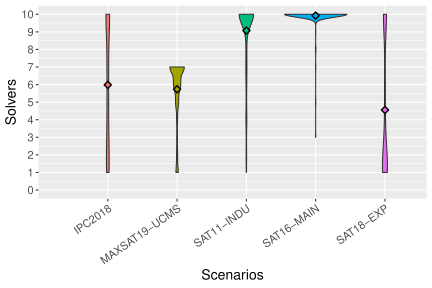
\includegraphics[width=0.5\linewidth]{plots/number_of_solvers_rf_kl.pdf}
    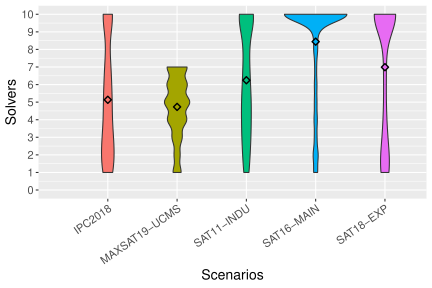
\includegraphics[width=0.5\linewidth]{plots/number_of_solvers_infjack_kl.pdf}
    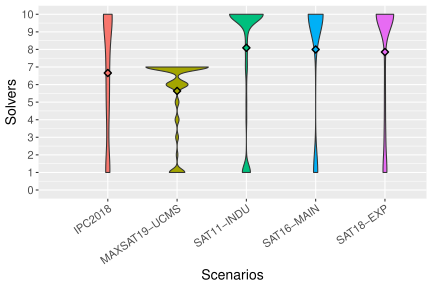
\includegraphics[width=0.5\linewidth]{plots/number_of_solvers_jack_kl.pdf}

    \caption[Distribution of Number of Selected Solvers when Using $AS_{kl}$]{
    Violin plot of the distribution of the number of selected solvers to run in parallel across all problem instances for each scenario for the respective optimal $kl$ and the maximum level of parallelism (seven processors for MAXSAT19-UCMS and 10 for all other scenarios). The diamond denotes the mean value. The top-left plot refers to the RFJ model, the top-right plot to the RI model, and the bottom plot to the RJ model.
    }
    \label{fig:numberofsolvers_kl}
\end{figure}


\section{Conclusions and Future Work}

In this study, we proposed a variation of the method introduced in Chapter 4 and expanded our experiments to incorporate these adaptations. We developed an alternative general approach for selecting solvers from a portfolio and scheduling them in parallel. This method leverages the predicted runtime distribution to make informed decisions about which solvers and how many to run in parallel. Specifically, in contrast to the method introduced in Chapter 4, where the joint probability of the prediction distribution is used as a measure of the likelihood that an algorithm performs, as well as the best-predicted solver, the new approach utilizes the KL divergence formula. This allows us to evaluate how much an algorithm's prediction diverges from the best-predicted solver, excluding solvers whose predictions differ the most. Moreover, similar to previous chapter, we measured the actual runtime when operating multiple algorithms in parallel, instead of relying on assumed sequential runtimes. 

Our results showed that while the previous method outperforms the new approach, in the absence of the old method, the new approach proves to be superior. Additionally, tuning the threshold for the joint probability in the method of the previous chapter varies significantly between different benchmarks and performance models. In contrast, the tuned threshold for divergence in the new approach is more consistent and this consistency can reduce the computational effort required for tuning.

For future work, we plan to explore replacing the performance models with models trained on parallel data instead of sequential data. Currently, the training data does not reflect the actual runtimes when algorithms are executed in parallel, and running algorithms in parallel can introduce overhead. We aim to evaluate whether this replacement improves portfolio selection performance.
  
% Cheat to bring in other references
%\nocite{*} % delete or comment this out.
